\documentclass[]{article}
\usepackage{geometry}
\geometry{
	a4paper,
	total={170mm,257mm},
	left=0.75in,
	top=0.75in,
	right=0.75in,
	bottom=1in,
}
\usepackage{gensymb}
\usepackage{lipsum}
\usepackage{graphicx}
\usepackage{caption}
\captionsetup{width=0.8\textwidth, justification=centering}
\usepackage{amsmath}
\usepackage[url=false,
backend=bibtex,
style=authoryear-comp,
doi=true,
isbn=true,
backref=false,
dashed=false,
maxcitenames=2,
maxbibnames=99,
natbib=true]{biblatex}
\addbibresource{bubbleBurstingVE.bib}
\DeclareNameAlias{author}{last-first}
\renewbibmacro{in:}{}
\usepackage{xcolor}
\usepackage[colorlinks,citecolor=blue]{hyperref}
\DeclareFieldFormat[article, inbook]{title}{#1}

\usepackage{fancyvrb}
\usepackage{siunitx}
\title{\textbf{Reply to Refree 2}}
\date{\vspace{-5ex}}
\newcommand{\AKD}[1]{{\textcolor{magenta}{#1}}}

\usepackage[textwidth=\dimexpr\textwidth-2cm\relax]{todonotes}
\makeatletter
\@mparswitchfalse%
\makeatother
\normalmarginpar %for right-handed notes and lines, or
\newcommand{\vsy}[1]{\todo[color=orange, bordercolor=none, textcolor=white]{Vatsal}\textcolor{orange}{#1}}

\newcommand{\sos}[1]{\todo[color=red, bordercolor=none, textcolor=white]{SOS}\textcolor{red}{#1}}

\newcommand{\oo}{\color{magenta} \normalfont}
\newcommand{\bb}{\color{black} \normalfont}

\newcommand{\vs}{\color{orange} \normalfont}


\renewcommand{\thefigure}{R2.\arabic{figure}}
\captionsetup[figure]{labelformat=default}

\begin{document}

\maketitle % This command prints the title, author, and date

We thank the referee for carefully reading our manuscript and providing valuable feedback and suggestions. We have reviewed the referee’s comments and made changes based on their suggestions. Below, we offer a point-to-point reply to each of the referee’s comments and include the changes made in the manuscript. The referee’s comments are in italics, and our replies are in plain black. Changes in the manuscript are highlighted in magenta.

\begin{enumerate}
    \item \textbf{\textit{The use of O-B to solve for drop formation and rupture.}}
 \begin{enumerate}
    \item
     \begin{itemize}
        \item  \textit{While it is acknowledged in the text, that O-B does not account properly for interface rupture and that it is not resolved properly in the simulations, that information is kind of buried and is missing from the introduction, abstract and conclusion.....In general, the physical discussion of the limits of O-B is missing in the paper......Again, no discussion on page 7 is provided on whether or not O-B is accurate to model rupture of visco-elastic liquids.}

        We understand the reviewer's concern about the discussion on limitations of the Oldroyd-B model.
        That is why, we dedicated a complete paragraph in section 2.1 to discuss the limitations of Oldroyd-B and also the reasons behind our choice. More details are then also mentioned in Section 3 (Results) and Section 5 (Conclusion \& Outlook). Based on the reviewer's suggestion, we have now added some information on the limitations of the Oldroyd-B model in the Introduction section.

        % \vsy{\#TODO-DONE: here, we yield and accept to change.. but in the next point, we will push back.. a little.}

        \item \textit{The present work very much calls for experimental validation (which can be done later) and this should be stated very clearly..........I would make the conclusions much more humble given the above remarks and the questions remaining in terms of lack of experimental validation. I think the present work is very nice and can serve as a road map, but until it is compared to experiments, the validity of O-B in the regime tested (especially for drop production) remains completely open. }

        % We agree with the reviewer that one should check how well the experiments are described by our simulation results. The need to compare experiments with current results has been mentioned in Section 5. For another ongoing project, we are working on it and hope to reveal the comparison between experiments and simulations.

        % \vsy{\#TODO-DONE: Additionally, we should highlight the point that OB still has all the essential Physics in. We are not trying to make a digital twin. Of course, for that, one will need to worry about the exact constitutive relation. the important thing here is: we take the leading order Physics: relaxation and application of stress when there is deformation and we do so by moving in the G-$\lambda$ parameter space. We agree 100\% with the reviewer that it is a good roadmap calling for future experiments and comparisons and refinement of the mode.}
     \end{itemize}

     We thank the referee for raising these important points about the use and limitations of the Oldroyd-B model in our study. We agree that limitation of Oldroyd-B need more prominence and the call for experimental validation should be stated very clearly. In the revised manuscript, we have more explicitly highlighted the limitations of the Oldroyd-B model in the Introduction and Conclusion. We also reiterate that this work should be viewed as a conceptual roadmap rather than a definitive quantitative prediction, and that future experimental validation and comparison with more advanced viscoelastic models are essential. We have also added an appendix to serve as a starting point of any further one-to-one comparison. Here are the changes made: 


     \begin{itemize}
        \item \S~1: \oo Despite its simplicity, we note that Oldroyd-B model has some crucial limitations.
        For instance, it cannot account for the shear-thinning behavior of polymer solutions and it predicts the divergence of stresses for strong extensional flows \citep{yamani2023master,alves2021numerical}.  
        Consequently, the Oldroyd-B model cannot accurately capture the final stages of filament thinning or the actual rupture of viscoelastic filaments, which may affect predictions of droplet detachment and fine aerosol formation.
        Nevertheless, we choose the Oldroyd-B model as its simplicity allows us to gain fundamental insight into the interplay between capillary, viscous, and elastic forces during bubble bursting.
%        \textcolor{cyan}{AO: Check my changes on this passage in the manuscript. Neglect this comment if you do not agree with the changes.}
        \bb\,
        \item \S~2.1: ``Additionally, the conformation tensor $ \boldsymbol{\mathcal{A}}$ relaxes to its base state $\boldsymbol{\mathcal{I}}$ over time due to thermal effects.
        Once more, using the Oldroyd-B model, $ \boldsymbol{\mathcal{A}}$ follows a linear relaxation law \oo (i.e., the rate of change of $\boldsymbol{\mathcal{A}}$ in the Lagrangian frame is linear in $\boldsymbol{\mathcal{A}}$),
%        \textcolor{cyan}{AO: Check my changes on this passage in the manuscript. Neglect this comment if you do not agree with the changes.}
        \bb\,

        \begin{align}
            \label{Aupperconv}
            \stackrel{\smash{\raisebox{0ex}{$\mkern8mu\boldsymbol{\nabla}$}}}{\boldsymbol{\mathcal{A}}}  =  - \frac{1}{De} \left( \boldsymbol{\mathcal{A}} - \boldsymbol{\mathcal{I}}  \right),
        \end{align}

        \noindent where

        \begin{align}
            \label{Aupper_def}
            \stackrel{\smash{\raisebox{0ex}{$\mkern8mu\boldsymbol{\nabla}$}}}{\boldsymbol{\mathcal{A}}} \equiv \frac{\partial\boldsymbol{\mathcal{A}}}{\partial t} + \left(\boldsymbol{u\cdot\nabla}\right)\boldsymbol{\mathcal{A}} - 2\text{Sym}\left(\boldsymbol{\mathcal{A}\cdot}\left(\boldsymbol{\nabla u}\right)\right)
        \end{align}

        \noindent is the frame-invariant upper convected Oldroyd derivative of second-rank tensor $\boldsymbol{\mathcal{A}}$, and $De = \lambda/\tau_\gamma$ (defined in equation~1.4) is the Deborah number, representing the ratio of the polymer relaxation time $\lambda$ to the process timescale $\tau_\gamma$ and Sym depicts the symmetric part of the tensor. \oo We note that while the Oldroyd-B model is nonlinear in terms of the velocity field and its gradient, both the stress term and its relaxation law remain linear in $\boldsymbol{\mathcal{A}}$. This characteristic contrasts with models such as the Giesekus model, which involves a quadratic term $\boldsymbol{\mathcal{A}\cdot\mathcal{A}}$ \citep{giesekus1982simple}, or the FENE models, which include a nonlinear term involving a finite-extensibility parameter $L$ \citep{bird1980polymer}. Therefore, the Oldroyd-B model is often referred to as ``quasi-linear”  \citep{davoodi2018secondary, alves2021numerical} \bb\,''
        \item \S~2.1: ``The Oldroyd-B model, despite its widespread use due to its simplicity, fails to capture several important physical phenomena \citep{snoeijer2020relationship}. It inadequately describes shear-thinning behavior in polymeric liquids \citep{yamani2023master} and erroneously predicts unbounded stress growth in strong extensional flows \citep{mckinley2002filament, eggers2020self}. 
        These limitations can be addressed by incorporating finite polymer extension, for example, by increasing the effective $Ec$ as the polymer approaches full extension \citep{hinch2021oldroyd,zinelis2023transition}. Various extensions of the Oldroyd-B equations have been developed to account for such nonlinearity, either in equations~(2.4) and~(2.5) or in the solvent contribution in equation~(2.3) \citep{de1974coil,tanner2000engineering,mckinley2002filament,alves2021numerical}. In this study, we employ the Oldroyd-B model to include the two primary effects of the polymer addition: the additional stress ($Ec$) and polymeric liquid memory ($De$) \citep{snoeijer2020relationship}. Our aim is to provide a comprehensive understanding of the entire $Ec$-$De$ parameter space (figure~1b).
        \oo 
        However, it is crucial to note that the Oldroyd-B model, while serving as a useful baseline, cannot accurately reproduce the finite-time breakup of viscoelastic filaments \citep{eggers2020self} or the full complexity of interface rupture \citep{lohse-2020-pnas}. These limitations warrant caution when interpreting the final stages of jet thinning and droplet formation, particularly in scenarios involving strong polymer stretching\bb.''
        \item \S~5: ``In conclusion, this study provides a comprehensive characterization of bubble bursting in viscoelastic media, interpreting the interplay between elastic, viscous, and capillary forces by moving in the $Oh_s$-$Ec$-$De$ phase space. 
        \oo
        As a starting point, we employed the Oldroyd-B constitutive model. While this choice elucidates the basic interplay of elasticity, viscosity, and capillarity, it does not capture shear-thinning effects or finite extensibility of polymer chains. Therefore, the predicted droplet sizes, jet thinning dynamics, and ultimate filament breakup must be interpreted with caution. More complex viscoelastic models (e.g., Giesekus, FENE-P) that incorporate finite extensibility and nonlinearities will likely alter certain details of our findings. Hence, our results should be viewed as a conceptual road map rather than definitive predictions. 
        An essential extension of our study involves the experimental validation of the numerical results. Controlled laboratory studies using polymer solutions with known rheological properties are needed to assess the accuracy of the Oldroyd-B model in this parameter regime (also see appendix~\ref{app:accounting}). Such comparisons will help determine where the simplified assumptions fail and guide refinements, including the use of more realistic constitutive equations.
        
        Despite these caveats, our study offers a foundation for understanding how viscoelasticity can either suppress or enhance droplet formation during bubble bursting. We hope this work will inspire future experiments and numerical explorations using more advanced rheological models, ultimately leading to a more complete and quantitative picture of viscoelastic bubble bursting across different application domains.
        \bb.''

        \item \oo
        \textbf{Appendix B. A note on the range of control parameters considered in this work}
        In this appendix, we tabulate and compare the range of dimensionless parameters explored in this work with those available in the literature on viscoelastic effects in bubble bursting. Tables~\ref{tab:ExpOnlydim_numbers} and \ref{tab:dim_numbers} summarize the physical properties and corresponding dimensionless numbers from three representative experimental studies.
        
        \begin{table}
            \begin{center}
                \begin{tabular}{lcccccc}
                    \hline
                    &$c$ & $R$ & $\eta_s$  & $\lambda$ & $\eta_p$ & $G$ \\
                    & (ppm) & ($\si{\milli\meter}$) & ($\si{\milli\pascal\second}$) & ($\si{\micro\second}$) & ($\si{\milli\pascal\second}$) & ($\si{\pascal}$) \\[3pt]
                    \citet{cheny1996extravagant} & [0, 100]  & 7.5, 19  & 300   & N/A & [0, 18] & N/A \\
                    \citet{rodriguez2023bubble} & [0, 350] & 1 & 1  & [0, 500] & [0, 0.5] & [0, 1] \\
                    \citet{cabalganteeffect} & [0, 100] & 0.93 & 0.89 & [0, 700] & [0, 2] &[0, 1] \\
                    \hline
                \end{tabular}
                \caption{Representative values of physical parameters in polymer solution studies from three representative works on the Worthington jets from the literature. Across these studies, the density of the medium and its surface tension coefficient are roughly $1000\,\si{\kilogram}/\si{\cubic\meter}$ and $70\,\si{\milli\newton}/\si{\meter}$, respectively. N/A represents unavailable data. See table~\ref{tab:dim_numbers} for the estimates of dimensionless numbers using these properties.}
                \label{tab:ExpOnlydim_numbers}
            \end{center}
        \end{table}
        
        \begin{table}
            \begin{center}
                \def~{\hphantom{0}}
                \begin{tabular}{lccccc}
                    \hline
                    & $Oh_s$ &  $De$ & $Ec$ & $Oh_p$ & $Bo$ \\[3pt]
                    This work & [10$^{-3}$, $10^0$] & [0, $\infty$) & [0, 10$^3$] & [0, $\infty$) & $10^{-3}$ \\
                    \citet{ari2024bursting} & [$10^{-3}, 10^{-2}$]  & [0, $10^2$] & [0, $10$] & [$10^{-3}, 10^{-2}$] & $10^{-3}$ \\
                    \citet{cheny1996extravagant}  & $10^{-1}$ & N/A & N/A & [0, $10^{-2}$] & [$10, 10^2$] \\
                    \citet{rodriguez2023bubble}  & $10^{-3}$  & [0, $10^{-1}$]& [0, $10^{-2}$] & [0, $10^{-3}$] & $10^{-1}$ \\
                    \citet{cabalganteeffect} & $10^{-3}$ &  [0, $2 \times 10^{-1}$] & [0, $10^{-2}$] & [0, $10^{-2}$] & $10^{-1}$ \\
                    \hline
                \end{tabular}
                \caption{Representative values of dimensionless numbers in this work as compared to those from previous studies. For experimental studies, the dimensionless parameters are calculated using the properties in table~\ref{tab:ExpOnlydim_numbers}. For \citet{ari2024bursting}, we have only considered the limiting cases of zero yield-stress. We note that while experiments are naturally limited in their accessible parameter ranges, our numerical study explores a broader range to establish comprehensive scaling laws and regime transitions.}
                \label{tab:dim_numbers}
            \end{center}
        \end{table}
        
        Table~\ref{tab:ExpOnlydim_numbers} presents key physical parameters including polymer concentration ($c$), bubble radius ($R$), solvent viscosity ($\eta_s$), polymer relaxation time ($\lambda$), polymer contribution to viscosity ($\eta_p$), and elastic modulus ($G$). The corresponding dimensionless numbers are shown in Table~\ref{tab:dim_numbers}, where we compare our parameter space with both experimental and computational studies from the literature. Our work systematically explores a significantly broader range of these parameters compared to experimental studies, which are often constrained by practical limitations in achievable polymer concentrations and relaxation times. This comprehensive coverage allows us to identify universal scaling laws and regime transitions that may be challenging to observe experimentally.
        
        The ranges explored in our numerical study suggest several promising directions for future experimental investigations. For instance, while moving in the $De$-$Ec$ parameter space, experiments could probe the robustness of our predicted transitions and scaling laws. Experimental studies would not only validate our computational findings but could also reveal additional physical mechanisms not captured by the Oldroyd-B model. We anticipate that trying new polymers and advances in characterization techniques \citep{gaillard2024beware} will continue to expand the experimentally accessible parameter space, enabling increasingly detailed comparisons between simulations and experiment.
        \bb
     \end{itemize}

        \item \textit{Moreover, the resolution used by the authors is quite coarse (levels 9, 10 and 11 in basilisk wording).......The Berny et al simulations for bubble bursting and the Turkoz et al simulations for visco-elastic thinning were performed up to level 14 (so a factor 8 better than what the authors do here) so the authors can very much increase their resolutions beyond what they did (and they should)..........I am surprised by the relatively coarse resolution used in the manuscript (for a 2d simulation). The authors need to demonstrate that these resolutions are enough for what they describe quantitatively in the manuscript......How do you understand physically the required grid size? Is it something like a number of grid point per capillary size? Viscous boundary layer?}

        % \vsy{\#TODO-DONE: find a funny comeback about this misunderstanding.. Must highlight that quoting the level of resolution means nothing.. it is essentially useless. In order to get similar results on a uniform grid, one would need $N = 2^{\text{Level}}/L_0$ cells across the unit length. And in fact, if you calculate that for both Berny and so on and us, we are using grids finer than Berny... do we go higher in resolution? check?}
        % The reviewer mentioned that the levels of resolution are 9, 10, and 11. But, we want to clarify that the levels of resolutions are 12, 13 and 14 instead.
        % Our simulations are refined and the solutions are grid-independent.
        % This misunderstanding could have been caused by the fact that we mentioned the minimum grid size to be $R_0/2048$ for the domain with size $8R_0 \times 8R_0$. The grid points (adaptive equivalent) would become $2048 \times 8$ and the level becomes 14. The minimum grid size of $R_0/2048$ represents that the length scale of the bubble radius has 2048 grids.

        We thank the reviewer for raising this point. The reference to levels 9, 10, and 11 likely stems from a misunderstanding in how we report resolution. Rather than specifying levels directly, we report $\Delta/R_0$: the minimum grid size relative to the bubble radius $R_0$. Indeed, simply specifying the maximum level of resolution is incomplete as Basilisk C sets $2^{\text{Max-level}}$ cells across one dimension of the computational domain $L_0$. So, we report $\Delta/R_0 = L_0/2^{\text{Max-level}}$. 
        Our standard resolution ensures at least $512$ cells across $R_0$, and for cases requiring higher accuracy, we have used up to $2048$ cells across $R_0$. In practice, this corresponds to refinement levels reaching of 12 and 14, respectively (using $L_0 = 8$). So, in fact, we also go to the same refinement levels as \citet{berny2020role,berny2021statistics,turkoz2018axisymmetric,turkoz2021simulation}. We realize that our grid refinement was perhaps unclear. We have modified the text for clarity.

        ``\S~2.2: \oo
        These resolutions are consistent with previous studies by \citet{berny2020role,berny2021statistics} on bubble bursting and \citet{turkoz2018axisymmetric,turkoz2021simulation} on visco-elastic thinning with a maximum level of resolution of 14 (for $\Delta = R_0/2048$ and domain size $L_0 = 8R_0$)\bb.''

        \item \textit{Also, the authors need to show their grid convergence study, since several of their conclusions rely on the weak statement that “everything has been checked”........ Can you show that result? I do not see the figure demonstrating this stated fact.}

        We thank the reviewer for highlighting the importance of demonstrating grid convergence, as several conclusions depend on the robustness of our numerical results. In response, we have now added Appendix C in the manuscript to demonstrate grid independence of our results.  

        \oo
\textbf{Appendix C. Grid sensitivity tests}
This appendix assesses the grid independence of our numerical results by examining two important metrics: (i) the predicted droplet size and (ii) the regime transitions. Ensuring grid convergence is crucial, especially if interface ruptures due to finite grid resolution in our numerical code \citep{lohse-2020-pnas,chirco2022manifold,kant2023bag}. 

Figure~\ref{fig:gis}(a) shows the relative error in predicted droplet size as a function of the number of grid points per initial bubble radius $R_0/\Delta$, where $\Delta$ is the minimum grid size. We focus on $De \to \infty$ as this case is particularly demanding, featuring slender filaments due to viscoelastic stresses. The error is calculated relative to the finest resolution ($R_0/\Delta = 2048$). 
The data exhibit approximately first-order convergence, indicated by the dashed line scaling as $(R_0/\Delta)^{-1}$. 
For our standard resolution of $R_0/\Delta = 512$, the relative error is approximately 6\%, decreasing to about 3\% at $R_0/\Delta = 1024$.

While droplet size convergence demonstrates improved numerical accuracy with increasing resolution, the determination of regime transitions between different flow behaviors provides an even more stringent test. These transitions are highly sensitive to the details of jet breakup. Figure~\ref{fig:gis}(b) displays the dimensionless elastocapillary number $Ec$ at the transition boundary for different grid resolutions. We find that for $(R_0/\Delta) \geq 1024$, the transition curves do not change, confirming that the scaling behaviors previously identified -- namely $Ec_d \sim De^{-1}$ for $De \ll 1$ and $Ec_d \sim De^0$ for $De \gg 1$ -- are robustly reproduced across all grid resolutions tested.

\begin{figure}
	\centering
	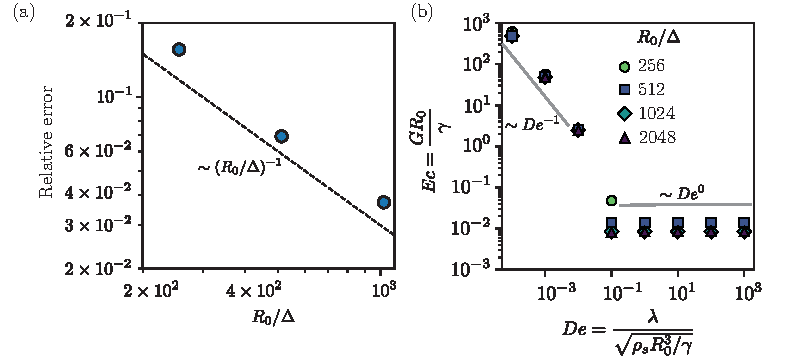
\includegraphics[width=\textwidth]{../Main/gridConverge-eps-converted-to.pdf}
	\caption{(a) Relative error in predicted droplet size versus the number of grid points per bubble radius, $R_0/\Delta$, at $De \to \infty$. The dashed line indicates a scaling of $(R_0/\Delta)^{-1}$, demonstrating approximately first-order convergence. (b) Dependence of the critical elastocapillary number $Ec_d$ at the dropping transition on the Deborah number $De$ for different grid resolutions ($R_0/\Delta = 256, 512, 1024, 2048$). The scaling behaviors $Ec_d \sim De^{-1}$ as $De \to 0$ and $Ec_d \sim De^0$ as $De \to \infty$ remain unchanged beyond $R_0/\Delta = 1024$.}
	\label{fig:gis}
\end{figure}

\bb

        % \sos{\#TODO-DONE: Ayush, can we add some of the plots regarding this point? Add two figures: (a) figure 8a but done with a zoo of grids and (b) $r_d(Ec, De \to 0)$.}

        \item \textit{...So the discussion in the paper is problematic since it is stated as if the determination of the rheology is a closed....No discussion of various other possible visco-elastic rheology are presented in the introduction. A small comment is given much later in the text. (page 7).}
        
        We thank the reviewer for this important observation regarding the discussion of rheological models. We agree that our original text may have suggested the determination of rheology was a closed problem. We have significantly revised the manuscript to address this concern in several ways:

        \begin{itemize}
            \item We now explicitly acknowledge that the Oldroyd-B model, while instructive and mathematically convenient, represents just one possible constitutive equation. We have added text clarifying that it does not incorporate nonlinear elastic effects or account for the finite extensibility of polymer chains.
        
            \item We have expanded the discussion of the model's limitations in Section 2.1, noting that ``The Oldroyd-B model, despite its widespread use due to its simplicity, fails to capture several important physical phenomena. It inadequately describes shear-thinning behavior in polymeric liquids and erroneously predicts unbounded stress growth in strong extensional flows."
            \item In the conclusions section, we have expanded our discussion of future research directions to include the exploration of more sophisticated rheological models.
            \item Wherever appropriate, we have mentioned a wide cateloge of possible extensions to Oldroyd-B that might be needed to compare against experiments.
        \end{itemize}

        These revisions better reflect the open nature of rheological modeling in complex fluids and acknowledge that our choice of the Oldroyd-B model represents a starting point rather than a definitive closure of the problem. We believe these changes address the reviewer's concern while maintaining the paper's focus on the fundamental physics of viscoelastic bubble bursting.

        % We understand the reviewer's point about the need to discuss viscoelastic rheological models, especially nonlinear models. We mentioned in Section 3 and Section 5 that extending the work to nonlinear viscoelastic models would be interesting. Based on the reviewer's suggestion, the following text has been added to the introduction.

        % \AKD{The estimation of rheological aspects of polymeric solutions is an open question. Work is ongoing to accurately model the viscoelastic flows (John et al. 2023, Yamani \& McKinely 2023, Gaillard et al. 2024).}

        % \vsy{\#TODO-DONE: we need to add a commentary (short) on what these different models are....}

        % We have already mentioned in Section 5 (Conclusion \& Outlook) about the need to understand the dynamics utilizing other complex rheological models. In the basilisk's numerical framework, it is easy to implement some of these models. The first step was to understand the behavior for $Oh_s-Ec-De$ parameter space. As a next step, effect of (third) rheological parameters should be understood.
    \end{enumerate}

     \item  \textbf{\textit{Implementation of O-B.}}
      \begin{enumerate}
          \item \textit{There are discussions in the basilisk community that the O-B implementation in basilisk fails for high Deborah numbers and recovers a Newtonian solution instead of an elastic one. It seems this issue has been solved by the authors but it is not clearly stated in the methods. When they state that they use Basilisk, if it is not the standard version (which is totally fine), they should say it clearly so that the user/community is aware of the advances they made and can use the proper version (i.e. the one the authors provide in their github).}

          \item \textit{I would also encourage the authors to discuss with the basilisk authors to integrate their contribution to the stable version, or at least as an alternative in the stable version.}

          \item \textit{Strangely, the authors do not cite (in the presentation of the numerical methods) other paper initially using/developing/implementing the O-B formulation in Basilisk. The work from Lopez-Herrera, Popinet \& Castrejón-Pita (2019, JFM) or Turkoz et al 2018 (JFM) should be cited, and there are probably more recent works using this implementation. The authors specifically use an implementation of the non-Newtonian rheology inside basilisk that is describe in certain paper and somehow these papers are not cited.}
      \end{enumerate}

      We thank the reviewer for their careful attention to the numerical implementation details.
      Yes, indeed, we have modified the standard basilisk version to accurately solve high Deborah numbers and shared it open source for anyone to use \citep{vatsalElastoFlow2024}. A well documented version of the code sufficient to reproduce the results reported in this paper is also available at \citet{Sanjay2024code}.
      As the reviewer suggested, clear statements on this are added to the updated version.

      \S~2.2: \oo
      To solve the Oldroyd-B viscoelastic constitutive relation (equation~(2.8)), Basilisk C uses the log-conformation method \citep{fattal2004constitutive} implemented by \citet{lopez2019adaptive} which has been used extensively at finite $De$ \citep{turkoz2018axisymmetric, turkoz2021simulation}. To explore the entire $Ec$-$De$ parameter space  (figure~1c), we have extended the log-conformation formulation to solve equations~(2.4) and~(2.5). In the spirit of Basilisk C, this code is detailed open-source at \citet{vatsalElastoFlow2024}.\bb\,

      We thank with the reviewer for encouraging us to integrate Basilisk C ElastoFlow \citep{vatsalElastoFlow2024} with the stable version. We will definitely do that.

      \item \textit{Not sure what the word “intriguingly” brings to the abstract.}

       The word is now removed from the abstract.

      \item \textit{It is very confusing that G and lambda in the abstract are both used for a quantity with dimensions and dimensionless. Non-dimensional numbers are not defined in the introduction. Abstract mentions three regimes depending on G and lambda but they do not specify the Oh (or La) range they are considering. As the authors know very well, drops will be observed in a certain range of Oh (or La) and cease to be emitted at low La (high Oh). They should clarify which range of Oh they consider and whether they explored various Oh in their parameter sweep in terms of G and lambda.}

	  We thank the reviewer for the comment. Based on their suggestion, we have rewritten the abstract.

	  Abstract:
      ``Bubble bursting and subsequent collapse of the open cavity at free surfaces of contaminated liquids can generate aerosol droplets, facilitating pathogen transport. After film rupture, capillary waves focus at the cavity base, potentially generating fast Worthington jets that are responsible for ejecting the droplets away from the source. While extensively studied for Newtonian fluids, the influence of non-Newtonian rheology on this process remains poorly understood.
      \oo
      Here, we employ direct numerical simulations to investigate the bubble cavity collapse in viscoelastic media, such as polymeric liquids.
      We find that the jet and drop formation are dictated by two dimensionless parameters: the elastocapillary number $Ec$ (the ratio of the elastic modulus and the Laplace pressure) and the Deborah number $De$ (the ratio of the relaxation time and the inertio-capillary timescale).
      We show that for low values of $Ec$ and $De$, the viscoelastic liquid adopts a Newtonian-like behavior, where the dynamics are governed by the solvent Ohnesorge number $Oh_s$ (the ratio of visco-capillary and inertio-capillary timescales).
      In contrast, for large values $Ec$ and $De$, the enhanced elastic stresses completely suppress the formation of the jet.
      \bb
      For some cases with intermediate values of \oo$Ec$ and $De$\bb, smaller droplets are produced compared to Newtonian fluids, potentially enhancing aerosol dispersal.
%      \textcolor{cyan}{AO: Check my changes on this passage in the manuscript. Neglect this comment if you do not agree with the changes.}
      By mapping the phase space spanned by \oo$Ec$, $De$, and $Oh_s$\bb, we reveal three distinct flow regimes: (i) jets forming droplets, (ii) jets without droplet formation, and (iii) absence of jet formation. Our results elucidate the mechanisms underlying aerosol suppression versus fine spray formation in polymeric liquids, with implications for pathogen transmission and industrial processes involving viscoelastic fluids.''

      \item \textit{Introduction: Page 4: “the full impact of these effects on bubble-bursting dynamics remains elusive”. Can the authors be more precise, they cite before this sentence a relatively large number of studies, including some of their own, so it would be helpful if the reader knew the key findings of these studies, and the gap in knowledge left that the authors wish to address in the present paper.}

      The text has been modified to make it more precise.

	``Given the potential for jet drops to transport pathogens or pollutants into the atmosphere, strategies to prevent their generation are pertinent. Recent studies unsurprisingly show that non-Newtonian effects, particularly that \oo viscoplasticity and\bb\, viscoelasticity, can suppress jet drop production \citep{sanjay2021bursting, sen2021retraction, rodriguez2023bubble, ji2023secondary}.
	While computational studies have successfully reproduced experimental observations, such as elasticity-induced droplet suppression \citep{cabalganteeffect, ari2024bursting}, the full impact of these effects on bubble-bursting dynamics remains elusive. \oo In this paper, we comprehensively answer the question: How does the viscoelasticity influence the observed regimes? What underlying physics governs the transitions between these regimes?\bb\,''

      \item \textit{Page 4 again: several quantities are not defined (like surface tension gamma, size of the bubble R0, etc). this is pretty sloppy. I know it is defined in the caption of figure 1 but it should also be defined in the text per JFM guidelines.}

      We agree with the referee that all quantities must be defined at their first occurrence in the paper. To ensure this, we define all of them at their first occurrence in the Introduction section (see page 2 of the revised manuscript). These definitions remain in the caption of Figure 1 for convenient reference. In our opinion, defining it once again on page 4 (when all quantities are already defined on page 2) would be unnecessary.

      \item \textit{I am not sure what figure 1a(i) brings since the numerical setup starts at figure 1a(ii).}

      We would like to keep figure 1a(i). For the process of bursting bubbles, particularly in a viscoelastic media, the initial conditions are critical. Also, it is also essential to know how this initial condition was achieved. For our work, we assume that the bubble sits at the liquid-gas interface for an infinite time (much larger than the relaxation time of the polymeric medium) before the cap bursts open leading to the collapse of the high surface energy cavity. This figure explicitly shows that we consider a bubble that has achieved equilibrium at the liquid-gas interface, where all elastic stresses have fully relaxed. We have now emphasized this assumption:

       \S~2.2:
       ``\oo We stress that here we assume that the bubble has resided at the liquid-gas interface for a duration far exceeding the polymeric medium's relaxation time, ensuring that elasticity does not influence the initial configuration \citep{ari2024bursting}.\bb\,
       During the bubble cap bursting, the film cap retracts almost instantaneously \oo(once again, we neglect the influence of elasticity)\bb, after which the capillary waves are generated.''

       This figure also establishes a reference configuration for future experimental validation, where different initial conditions could be incorporated based on experimental observations. We have now also expanded on this aspect in conclusion and outlook:

       \S~5:
       ``\oo Indeed, a critical assumption of this work is the initial condition and its history, particularly for bubbles at liquid-gas interfaces in viscoelastic or elastoviscoplastic media. Our current work assumes the bubble has resided at the interface for a duration far exceeding the polymeric medium's relaxation time, ensuring elastic stresses have fully relaxed before bursting. This idealized scenario provides a well-defined starting point but may not fully capture experimental conditions \citep{cheny1996extravagant,deoclecio2023drop}.\bb''

       We think that figure 1a(i) provides essential context for both our numerical methodology and future experimental comparisons and should be included in the present paper.

%      ..... \vsy{\#TODO-DONE: need a stronger reply here.}

%       We agree that the numerical simulations begin with the instant shown in Figure 1a(ii). Figure 1a(i) has been provided for a better understanding of the readers who might not be familiar with the problem beforehand. Figure 1a(i) illustrates how a bubble approaching the interface would make a thin liquid film and would cause an open bubble cavity, which is shown in Figure 1a(ii).

      \item \textit{Bubble bursting scaling laws: The authors do not cite the Ganan-Calvo 2017 PRL which remains the first one to propose a scaling law adequately representing the velocity and size of the drops ejected bubble bursting and jet drop formation. They only cite the similar work/analysis by Gordillo and co-authors.}

       We apologize for the oversight. Although Ganan-Calvo and Gordillo's theories rely on different underlying principles, they yield identical scaling predictions. However, this is not the place to favor one theory over the other as our main focus is to extend the physical understanding of this process to viscoelastic medium. We have now cited Ganan-Calvo 2017 PRL as well.

      \item \textit{“exact solutions for the first droplets’ size rd are well understood (see appendix A and Blanco-Rodrıguez \& Gordillo (2020)”: I would not call the work from Gordillo and exact solution, their theory is full of adjusted parameters, and so while it describes very well the data, it is more a scaling argument than a theory. The prefactors are not predicted by Gordillo, they are fitted to the data (experimental and numerical). Same for the Ganan-Calvo version of the work. It is however true, that this part of the problem is very well understood.}

      We thank the reviewer for this careful observation. We agree with the them. Based on their suggestion, to avoid any confusion, we have now replaced the `exact solutions' with `predictions'.

      \S~3.1:
      ``For Newtonian liquids, \oo predictions\bb\, for the first droplets' size $r_d$ are well understood (see appendix~A and \cite{ganan2017revision,blanco2020sea}).''

       \item \textit{Figure 4 shows qualitatively the drop size as a function of the non-dimensional parameters. Can you be quantitiatve in showing graphs? How well resolved would be the curve of drop size as a function of Ec at fixed Ohs? Can you quantify the deviation from the Newtonian case? Same question for the jet length, which also has a theoretical prediction from the Ganan-Calvo or Gordillo scaling laws (see Lai, Eggers and Deike, 2018 PRL for example). Same question regarding figure 6.}

       Notably, $r_d$ remains independent of $Ec$ and equal to Newtonian solutions, i.e., no deviations, until $Ec$ is not very close to the transition values. We have now highlighted this point in the text as well.

		\S~3.1:
        ``While $r_d$ follows the same trend with $Oh_s$ \oo observed at Newtonian limits\bb\, and remains invariant of $Ec$ below critical values..."
		\S~3.2:
        ``Figure 6(b) maps the $r_d$, showing $Ec$-independent droplet sizes \oo that are equal to values at the Newtonian limit\bb, until near the transition point....."

        We agree that the dependence of jet length on $Oh_s$ and their theoretical predictions has been studied in the past (as also pointed out by the referee). While $r_d$ remains independent of $Ec$, the jet length is observed to depend on $Ec$, $De$ and $Oh_s$. Given the added complexity posed by viscoelasticity, we didn't attempt to theoretically model the jet length. We have now added this aspect as a possible future scope.

        To quantify the deviation from the Newtonian asymptote, we have also added appendix D in the revised manuscript. 

        \oo
        \textbf{Deviation from the Newtonian asymptote}

        \begin{figure}
            \centering
            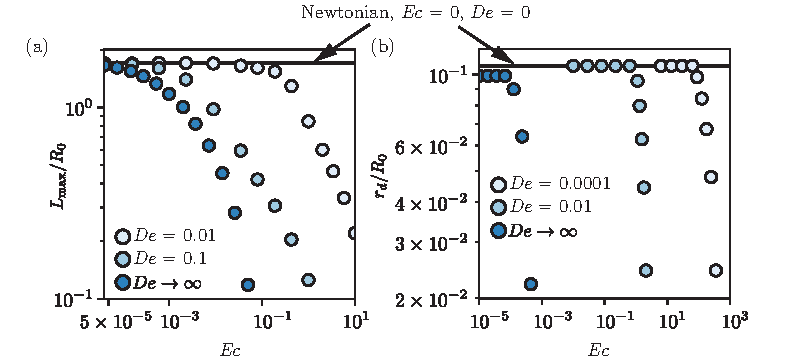
\includegraphics[width=\textwidth]{../Main/LMaxRd-eps-converted-to.pdf}
            \caption{{\oo Comparison of (a) maximum jet length $L_{\text{max}}/R_0$ and (b) first droplet size $r_d/R_0$ against the elastocapillary number $Ec$ at various Deborah numbers $De$ in the limit of $Oh_s \ll 1$. The horizontal lines indicate the Newtonian reference values (obtained at $Ec=0$). At small $Ec$, both $L_{\text{max}}$ and $r_d$ coincide with their Newtonian counterparts, demonstrating negligible viscoelastic influence. As $Ec$ increases beyond critical values, significant deviations from the Newtonian limits emerge, with the degree of departure depending on $De$. These results quantify the onset and magnitude of elastic effects relative to the Newtonian baseline, providing a clear framework for interpreting viscoelastic modifications to bursting bubble dynamics.\bb}}
            \label{fig:devNewt}
        \end{figure}

        In the main text, we showed that for small elastocapillary numbers $Ec$, the droplet size $r_d$ and jet length $L_{\text{max}}$ closely match those of the Newtonian case at arbitary $Oh_s$ (solvent Ohnesorge number) and $De$ (Deborah number). Only when $Ec$ approaches or exceeds critical values do we observe significant departures from the Newtonian reference.

        Figure~\ref{fig:devNewt} quantifies these deviations by comparing both the maximum jet length $L_{\text{max}}$ (Figure~\ref{fig:devNewt}a) and the first droplet size $r_d$ (Figure~\ref{fig:devNewt}b) against $Ec$ at various $De$, in the limit of $Oh_s \ll 1$. The symbols represent numerical results for the viscoelastic system, while the horizontal lines mark the corresponding Newtonian asymptotes (i.e., $r_d$ and $L_{\text{max}}$ values obtained at $Ec=0$). For small $Ec$, both $r_d$ and $L_{\text{max}}$ are invariant, indicating that viscoelastic stresses are negligible in this range. As $Ec$ increases and approaches the critical thresholds identified in \S~4, deviations emerge, ultimately leading to suppressed jetting or droplet formation.

        Notably, the critical $Ec$ value at which $r_d$ and $L_{\text{max}}$ deviate from their Newtonian counterparts depends on $De$. For high $De$, even a moderate increase in $Ec$ can trigger significant changes, reflecting the persistent elastic memory in the fluid. In contrast, for $De \ll 1$, where the polymeric stresses relax rapidly, larger $Ec$ values are necessary to produce noticeable departures from Newtonian behavior. Similarly, the Newtonian limit is readily recovered by reducing either $Ec$ or $De$ to zero.

        These results highlight that any interpretation of viscoelastic bubble-bursting dynamics should be framed with reference to the Newtonian baseline (either $De = 0$ or $Ec = 0$). By systematically mapping out these deviations, one can pinpoint the onset of non-Newtonian behavior and interpret observed jetting or droplet formation regimes as outcomes of either weak or strong elastic effects, all benchmarked against the Newtonian scenario.
        \bb

        % \sos{\#TODO-DONE: We must show $r_d(Ec)$ and $L_j(Ec)$ at different $Oh_s$ and $De$, respectively. It will be repetitive to do so in the paper (given that we already have the contour plots)--we must still give it as a plot in the review and rewrite this part accordingly. @Ayush: please take care of this.}

       \item \textit{Figure 8a and b. The authors say the transition from jet- no jet is independent of $Oh_s$. I believe them but they should show that the data overlap for all the $Oh_s$. Otherwise, it is confusing since the figure 7 shows a very clear dependence in $Oh_s$.}

      We have updated figure 8a and b to emphasize the $Oh_s$-independence as suggested by the referee (see figure~\ref{fig:transitionJets}.).

      \begin{figure}
      	\centering
      	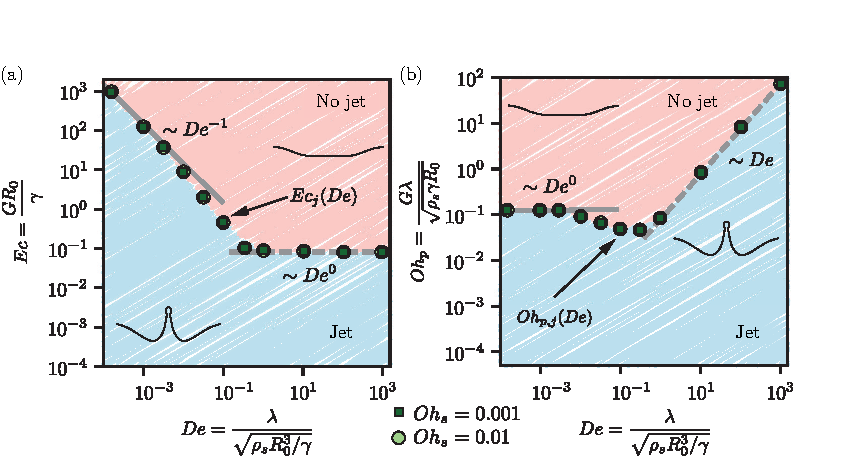
\includegraphics[width=0.75\textwidth]{../Main/Transtion_08_OnlyJet-eps-converted-to.pdf}
      	\caption{{\oo (a) The elastocapillary-Deborah number ($Ec$-$De$) and (b) the polymeric Ohnesorge-Deborah number ($Oh_p$-$De$) phase map delineating the transition between the regimes: (ii) jets without droplet formation and (iii) absence of jet formation. The data points represent the $Oh_s$-independent critical elastocapillary number $Ec_j(De)$ at which this transition occurs. The transition behavior exhibits distinct characteristics in different limits: as $De \to \infty$, the transition occurs at a constant $Ec$ (see gray dashed line showing $Ec_d \sim De^0$), while for $De \to 0$, the transition occurs at constant $Oh_p$ (see gray solid line showing $Ec_d \sim De^{-1}$, i.e., $Oh_{p,d} \sim De^0$).\bb}}
      	\label{fig:transitionJets}
      \end{figure}

      \item \textit{Figure 12b seems to show that the jet radius does not vary much with De, as compared to the Newtonian case. Since the jet radius will set the drop size (see Ganan-Calvo 2017), does this means that the drop size does not vary much with De? Is that coherent with the figures 4 and 6 in the paper.}

      We appreciate this insightful observation regarding the jet radius behavior in figure 12b. Let us clarify the connection to figures 4 and 6.

      The jet radius behavior shown in Figure 12b specifically examines the regime where $De \to 0$ and at a fixed $Oh_s = 0.01$. In this limit, the polymeric liquid effectively behaves like a Newtonian fluid with enhanced viscosity $\eta_{\text{effective}} = 3\eta_s + 2G\lambda$. This behavior differs from what is observed in figures 4 and 6, which examine different regions of the parameter space:

      \begin{itemize}
      	\item Figure 4 examines the $De \to \infty$ limit, where polymeric stresses persist indefinitely and elastic effects dominate. Here, both jet radius and drop size show strong dependence on $Ec$ in the vicinity of $Ec_j$ and $Ec_d$, respectively.
      	\item Figure 6 explores a fixed $De = 0.01$, which is at the edge of the zero $De$ limit and the effective $Oh$ argument works here. In this case, the $Oh_p$ dependence of figure 12b is equivalent to the $Ec$ dependence ($Ec = Oh_p/De$).
      	\item Figure 12b specifically shows the $De \to 0$ limit where polymers act effectively as additional viscosity. Here, the jet radius follows Newtonian-like scaling with $Oh_{\text{effective}}$ until reaching a critical $Oh_{p,c}$, beyond which bubble entrainment occurs.
      \end{itemize}

      This apparent independence of jet radius on $De$ in figure 12b is thus regime-specific and should not be interpreted as contradicting the broader parameter dependencies shown in figures 4 and 6. The different behaviors across these regimes reflect the rich physics of how polymeric relaxation timescales interact with the characteristic timescales of jet formation and breakup.

      We have modified the text accordingly:

      \S~4.2.2: ``\oo At small $Oh_p$, we observe that the jet radius maintains a value comparable to the Newtonian reference case (figure~12a: $Oh_p = 0, 0.005$). This behavior is consistent with the $De \to 0$ limit, where polymeric additives primarily contribute enhanced effective viscosity. Since the jet radius determines the resulting drop size \citep{ganan2017revision,blanco2020sea}, this independence of jet radii in the low $Oh_p$ regime suggests minimal variation in droplet size distribution compared to Newtonian cases.\bb''


%	\vsy{Yes, the jet radius does not vary much with $De$ in the limit of $De \to 0$ as shown in figure 12b. Notably, in this limit, the dimensionless polymeric viscosity dictates the jet radius and subsequently the drop size. However, we caution against comparison with figures 4 and 6--both are at fixed $De$ of $\to \infty$ and $0.01$, respectively. However, the apparent $De$-independence is only for $De \to 0$ in figure 12b.  \#TODO-DONE: needs refinement.}
%       We agree that the plot of jet radius against $Oh_p$ (Figure 12b) doesn't vary much with $De$. Contrarily, Figure 4 and 6 show the variation of drop size with $Ec$. Notably, $r_d$ remains independent of $Ec$ below the transition values $Ec_d$. Where $Ec_d$ depends on $De$ as shown in Figure 8. Thus, if $De$ and $Ec$ are within the regime where the drops are observed, then $r_d$ remains independent of $De$ and $Ec$ and only depends on $Oh_s$.

 \end{enumerate}

\printbibliography
\end{document}
